In order to study the effect of the variations of the frequency $f_c$ and the amplitude $A_u$ of the input $u_e$ on the second and third order harmonic distortion, we have computed $d_2$ and $d_3$ for a range of $A_u$ and $f_c$. The results can be seen on the figure \ref{fig:d2d3}. According to the graphic, the variations of the amplitude of the input do not affect the shape of the distortion levels. The amplitude has only an impact on the value of the distortion from 20 to 60 Hz. If it doubles, the pourcentage of the distortion will also be multiplied by two. On the other hand, when the fundamental frequency increases, the distortion levels $d_2$ and $d_3$ are stabilising at low values, nearly 0\% for $d_3$. It can be explained by the fact that the more the fundamental frequency grows, the more the harmonic pikes will be far from it as they correspond to $nf_c$. Their amplitude will be affected and will become of minor importance in front of the amplitude of the fundamental pike.

\begin{figure}[H]
 \centering 
 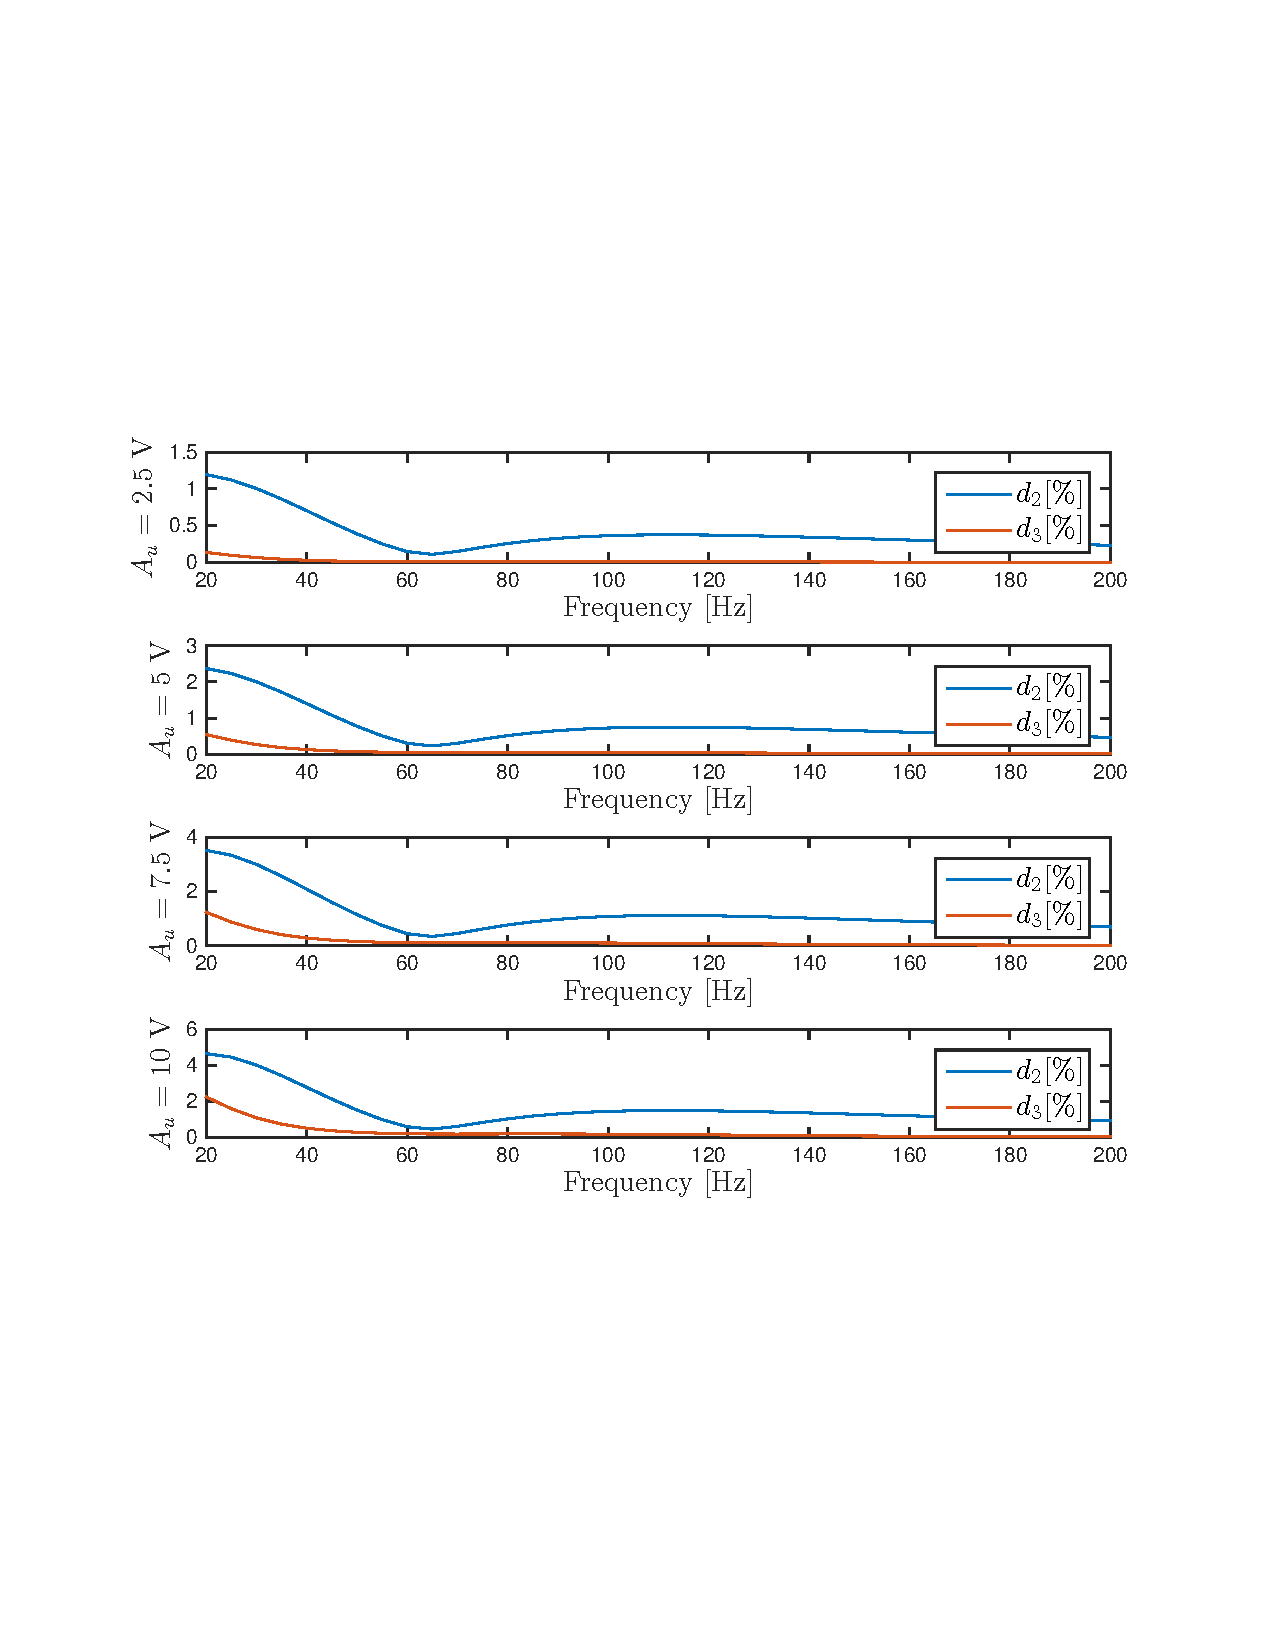
\includegraphics[trim=2cm 7cm 2cm 7cm, clip=true, totalheight=0.35\textheight, angle=0]{figures/P5d2d3.pdf}
 \caption{Effect of the variations of the frequency $f_c$ and the amplitude $A_u$ of the input $u_e$ on the second and third order harmonic distortion}
 \label{fig:d2d3}
\end{figure}